\section{Durchführung}
\label{sec:Durchführung}
Vor den Messungen werden für diesen Veruch drei periodische Funktionen gewählt und in eine Fourierreihen nach Gleichung \eqref{eq:gl1} entwickelt.
\subsection{Fourier-Transformation}
Diese Funktionen werden dann mit einem mit einem Funktionsgenerator erstellt und auf einem digitalen Oszilloskop ausgelesen.
Der Grundaufbau für diesen Versuch ist in Abbildung \ref{fig:aufbau} dargestellt.
\begin{figure}[H]
    \centering
    \caption{Versuchsaufbau für die Transformation eines Signals.}%\cite{v351}}
    \label{fig:aufbau}
    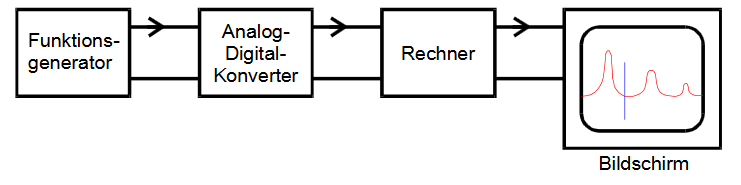
\includegraphics[width=\textwidth-20em]{content/aufbau.png}
\end{figure}
\noindent
Das Oszilloskop transformiert das eingehende Signal und wirft das Frequenzspektrum auf den Bildschirm.
Da über einen endlichen Zeitraum integriert wird ist das Linienspektrum unschärfer als Abbildung \ref{fig:lspek} darstellt.
Die Koeffizienten sind nicht als $\delta$-Distributionen zu erwarten, sondern als Linien endlicher breite.
Für die drei entwickelten Funktionen werden mit einem "Cursor" die ersten neun nicht verschwindenen Koeffizienten gemessen.
\subsection{Fourier-Synthese}
Für die Fourier-Synthese wird eine Oberwellengenerator verwendet. Dieser liefert eine Vielzahl an Sinusspannungen, welche Phasenstarr miteinander gekoppelt sind und deren Frequenzen sich wie ganze Zahlen verhalten.
Über Lissajou-Figuren wird die Phasenbeziehung zwischen den Koeffizienten überprüft.
Dafür wird die Grundschingung und die $n$-te Oberwelle an einem Oszillographen angeschlossen.
Dieser wird dann auf den $XY$-Betrieb geschalten.
Dort kann dann über die entsprechende Lissajou-Figur das gewünschte Verhältnis eingestellt werden.
Ist dies geschehen werden die ersten zehn Amplituden der Oberwellen entsprechend der errechneten Koeffizienten eingestellt.
Der "Summenschwingungsausgang" wird an den Oszillographen angeschlossen.
Das so enstandene Bild auf dem Oszillographen ist dann eine Überlagerung der Oberwellen.
 
